\documentclass[../main.tex]{subfiles}
\graphicspath{{\subfix{../IMAGES/}}}

\begin{document}
\localtableofcontents
La production dans les pays représente environ $25\%$ du PIB. De plus, elle représente $40\%$ du prix de revient d'un objet.\\

Un procédé de production est une opération de transformation qui permet de passer du matériaux brute à une pièce plus complexe à l'aide d'outils et d'énergie.\\
\warning Une opération d'assemblages ni un traitement thermique n'est un procédé de production.\\

Il existe trois classes de procédés de production :\\
\begin{enumerate}
    \item \textbf{ablatifs :} enlèvement de matière (fraisage/électro-érosion/usinage électrochimique);\\
    \item \textbf{réplicatif :} par ajout/déformation de matière dans un \textbf{outil de forme} qui a une forme dédiée (injection plastique/fonderie/forgeage/extrusion/emboutissage);\\
    \item \textbf{additif :} ajout de matière sans utilisation d'outil de forme (impression 3D).\\
\end{enumerate}

\subsection{Propriétés mécaniques des matériaux}
\quad \underline{Traction uniaxiale :} force quasi-statique. \\
Pendant la déformation, la force passe de $F'$ à $F'+dF'$ et la barre s'allonge de $dl'$ : \textbf{accroissement relatif de longueur : $\frac{dl'}{l'}$}\\
On a la somme des accroissements relatifs sur toute l'expérience :\\
\begin{itemize}
    \item \textbf{taux de déformation réel :} $\varepsilon = \int \frac{dl'}{l'} = \ln(\frac{l}{l_0}) = \ln(1+e)$\\
    \item \textbf{taux de déformation nominal :} $e = \frac{l-l_0}{l_0} = \int \frac{dl}{l_0}$\\
\end{itemize}

On appelle aussi \textbf{l'allongement relatif : $\frac{l}{l_0}$}\\
\warning $e\geq \varepsilon$\\

\warning Le taux de déformation réel est additif, pas le nominal.\\
Soit la contrainte réelle : $\sigma(\varepsilon) = \frac{F}{S}$, ne dépend que de l'allongement relatif.\\

\subsubsection{Élasticité}
\quad \underline{Si $\varepsilon<\varepsilon_e$ : élasticité :}\\
$\varepsilon_e$ : taux de déformation réel en limite élastique. Si $\sum \varepsilon_i < \varepsilon_e$ alors :\\
\begin{equation}
    \sigma(\sum \varepsilon_i) = \sum \sigma(\varepsilon_i)
\end{equation}
On a donc une relation linéaire et la relation exacte est donnée par : $\sigma(\varepsilon) = E\varepsilon$. \\
D'un autre côté, la loi approximative $\sigma = Ee$ surestime la contrainte réelle.\\

Au moment où $\sigma_e = E \varepsilon_e$, les dislocations commencent à bouger (seul le cisaillement fait bouger les dislocations)\\

$\sigma_e$ dépend du matériaux et de son état d'écrouissage. Celle ci peut augmenter par plusieurs moyens :\\
\begin{itemize}
    \item On écrouit et augmente la densité des dislocations\\
    \item on raffine la micro-structure : plus de joints de grains augmente la limite élastique\\
    \item on peut aussi rajouter des éléments d'alliages pour bloquer les dislocations\\
\end{itemize}

\subsubsection{Plasticité}
La loi de Hooke n'est plus valable\\
Il existe des loi approximative différentes par matériaux : les lois d'écrouissage\\
Une loi applicable pour beaucoup de matériaux revenus : \\
\begin{equation}
    \sigma = K \varepsilon^n
\end{equation}
C'est la \textbf{loi de Ludwik}\\
On a n le coefficient d'écrouissage et K le module d'écrouissage [K] = MPa\\

Par continuité entre le domaine élastique et plastique :\\
\begin{equation}
    K = E\varepsilon_e^{1-n}
\end{equation}

\subsubsection{Relaxation}
On laisse ici revenir la force à 0. \\
On a la relation $E = \frac{\sigma_r}{\varepsilon_r-\varepsilon_p} = \frac{E \varepsilon_e^{1-n}\varepsilon_r^n}{\varepsilon_r-\varepsilon_p}$\\
Loi de la déformation permanente : \\
\begin{equation}
    \frac{\varepsilon_r}{\varepsilon_e} - (\frac{\varepsilon_r}{\varepsilon_e})^n = \frac{\varepsilon_p}{\varepsilon_e}
\end{equation}
Pour trouver $\varepsilon_r$, on trouve la limite de la suite $x_{m+1} = \frac{\varepsilon_p}{\varepsilon_e}+x_m^n$, $x_0 = 0$. Ensuite, $\varepsilon_r = \varepsilon_e \overline{x}$\\

\subsubsection{Écrouissage}
Il s'agit d'une pièce ayant subi une traction jusqu'en zone plastique. Le taux de déformation réel $\varepsilon'$ du matériaux écroui est une fonction du taux de déformation réel de l'échantillon depuis l'état initial. Soit $l_0$ la longueur initiale et $l_p$ la longueur écroui. \\
$\varepsilon = \ln(\frac{l}{l_0})$, $\varepsilon' = \ln(\frac{l}{l_p})$, $\varepsilon_p = \ln(\frac{l_p}{l_0})$\\
Équation de transfert :\\
\begin{equation}
    \varepsilon = \varepsilon'+\varepsilon_p
\end{equation}
\warning Pas vrai avec les e : $e' = \frac{l-l_p}{l_p}$, $e_p = \frac{l_p-l_0}{l_0}$ et $e = \frac{l-l_0}{l_0} = e_p + (1+e_p)e'$\\

On a maintenant, $\varepsilon_e' = \varepsilon_e^{1-n} \varepsilon_r$\\
$\sigma_e' = (\frac{\varepsilon_r}{\varepsilon_e})^n\sigma_e$\\
Pour l'échantillon écroui, on a la loi de \textbf{Swift} (Ludwik décalé) :\\
\begin{equation}
    \sigma = K\varepsilon^n = K(\varepsilon_p + \varepsilon')^n
\end{equation}
Taux d'écrouissage : $\varepsilon_p$\\

Comme $\varepsilon_e' > \varepsilon$, l'écrouissage augmente : le taux de déformation réel en limite élastique, la limite élastique et la dureté.\\
\warning n et K sont des invariants d'écrouissage!\\

On peut réécrire les coefficients : \begin{itemize}
    \item $K = E \frac{\varepsilon_e}{(\varepsilon_e+a)^n}$, $\varepsilon_e$ la valeur de la limite élastique écrouie\\
    \item $(\varepsilon_p+a) = (\varepsilon_e+a) - \varepsilon_e (\frac{\varepsilon_r+a}{\varepsilon_e+a})^n$\\
    \item $\hat{\varepsilon}_e = \sqrt[1-n]{\frac{\varepsilon_e}{(\varepsilon_e+a)^n}} $\\
    \item $\frac{\varepsilon_p+a}{\hat{\varepsilon}_e} = \frac{\varepsilon_r+a}{\hat{\varepsilon}_e} - (\frac{\varepsilon_r+a}{\hat{\varepsilon}_e})^n$\\
    \item Les rapports de rayon, section et volumes ne changent pas pour Poisson et Considère. Pour Hencky cependant : $\frac{r}{r_0} = e^{(\frac{1}{2}-\nu)\varepsilon_e (\frac{\varepsilon+a}{\varepsilon_e+a})^n-\frac{1}{2}\varepsilon}$, $\frac{S}{S_0} = e^{(1-2\nu)\varepsilon_e (\frac{\varepsilon+a}{\varepsilon_e+a})^n-\varepsilon}$, $\frac{V}{V_0} = e^{(1-2\nu)\varepsilon_e (\frac{\varepsilon+a}{\varepsilon_e+a})^n}$
\end{itemize}

\subsubsection{Rupture}
Définition des valeurs :\\
$\varepsilon_{ult}$ : taux de déformation réel en rupture (descente droite), associée avec $\sigma_{ult}$\\
$\varepsilon_{p;ult} = \varepsilon_{ult}-\varepsilon_e^{1-n}\varepsilon_{ult}^n$ le taux réel de rupture permanent\\

\subsubsection{Loi de Poisson}
L'échantillon reste cylindrique pendant que son rayon diminue (on ne prend pas en compte la striction). \\
\warning Uniquement en élasticité\\
\begin{equation}
    \frac{dr}{r} = -\nu \frac{dl}{l} \Rightarrow r = r_0 (\frac{l}{l_0})^{-\nu} = r_0 e^{-\nu \varepsilon}
\end{equation}
Dans la traction, la longueur et le volume augmentent toujours. \\
$R_m = Kn^n e^{(1-2\nu)\varepsilon_e-(n-a)}$, $\varepsilon_m = n-a$


\subsubsection{Théorie de Considère}
On suppose ici que V est constant dans la zone plastique.\\
Cependant, cette théorie est inconsistante car si écrouissage, on obtient $V_p < V_0$\\
Elle reste tout de même proche de la réalité si n est proche de 0.\\

\subsubsection{Théorie de Hencky}
On résout ici le problème de la théorie de Considère, cependant plus compliqué à utiliser, on ne la prend pas souvent en compte.


\begin{table}[hbt!]
    \centering
    \begin{tabular}{||c|c|c|c|}
    \hline
         & Elasticité & \multicolumn{2}{c|}{Plasticité}\\
         \hline
        Relation & Poisson & Considère & Hencky\\
        \hline
        $\frac{r}{r_0}$ & $e^{-\nu \varepsilon}$ & $e^{(\frac{1}{2}-\nu)\varepsilon_e - \frac{\varepsilon}{2}}$ & $e^{(\frac{1}{2}-\nu)\varepsilon_e(\frac{\varepsilon}{\varepsilon_e})^n - \frac{\varepsilon}{2}}$\\
        $\frac{S}{S_0}$ & $e^{-2\nu \varepsilon}$ & $e^{(1-2\nu)\varepsilon_e - \varepsilon}$ & $e^{(1-2\nu)\varepsilon_e (\frac{\varepsilon}{\varepsilon_e})^n - \varepsilon}$\\
        $\frac{V}{V_0}$ & $e^{(1-2\nu)\varepsilon}$ &$e^{(1-2\nu)\varepsilon_e}$ & $e^{(1-2\nu)\varepsilon_e (\frac{\varepsilon}{\varepsilon_e})^n}$\\
        \hline
    \end{tabular}
    \caption{Récapitulatif}
\end{table}
\warning Ne dépendent pas de l'écrouissage : il suffit d'adapter $\varepsilon_e$ à celui de l'écrouissage. \\

\subsubsection{Forces et courbes de traction}
Contrainte nominale : $R = \sigma(\varepsilon) s(\varepsilon) = \frac{F}{S_0} = \frac{\sigma S}{S_0}$\\
Contrainte réelle : $\sigma = \frac{F}{S}$\\

En élasticité : $R = E \varepsilon e^{-2\nu}$.\\
En plasticité : $R=K\varepsilon^n e^{(1-2\nu)\varepsilon_e - \varepsilon}$\\

\underline{Cas général :} $\varepsilon_e \leq n \leq \varepsilon_{ult}$\\
alors la résistance atteinte pendant l'écrouissage. Pour un matériaux revenu et sous hypothèse de considère :\\
$\varepsilon_m = n$, $R_m = K(\frac{n}{e})^ne^{(1-2\nu)\varepsilon_e}$\\

\underline{Cas fragile :} $n >\varepsilon_{ult}$ la résistance est atteinte à la rupture. \\
$\varepsilon_m = \varepsilon_{ult}$, $R_m = \sigma_{ult} e^{(1-2\nu)\varepsilon_e - \varepsilon_{ult}}$\\

\underline{Cas matériau dur :} $n < \varepsilon_e$ alors la résistance dans zone élastique vaut :\\
\begin{itemize}
    \item si $\varepsilon_e < \frac{1}{2\nu}$ alors $R_m = R_e$, $\varepsilon_m = \varepsilon_e$\\
    \item si $\varepsilon_e \geq \frac{1}{2\nu}$ alors $R_m = \frac{E}{2\nu e}$, $\varepsilon_m = \frac{1}{2\nu}$\\
\end{itemize}

\subsubsection{Fonction de traction}
Le module d'écrouissage K est lié à la résistance $R_m$. On a donc les relations :\\
\begin{itemize}
    \item Pour un matériaux revenu : \begin{itemize}
        \item $K = R_m (\frac{e}{n})^n e^{-(1-2\nu)\varepsilon_e}$\\
        \item $R = \begin{cases} E\varepsilon e^{-2\nu \varepsilon} & \varepsilon \leq \varepsilon_e\\ R_m(\frac{\varepsilon}{n}e^{1-\frac{\varepsilon}{n}})^n & \varepsilon \geq \varepsilon_e\\
        \end{cases}$
    \end{itemize}
    \item Pour un matériaux écroui : \begin{itemize}
        \item $R = \begin{cases}E\varepsilon' e^{2-\nu \varepsilon_e'} & \varepsilon\leq \varepsilon_e\\ R_m'(\frac{a+\varepsilon'}{n} e^{1-\frac{a+\varepsilon'}{n}})^n & \varepsilon \geq \varepsilon_e            
        \end{cases}$
        \item $R_m' = e^{a+(1-2\nu)(\varepsilon_e'-\varepsilon_e)R_m}$\\
        \item On a le taux d'écrouissage $a$ ainsi que $\varepsilon=\varepsilon'+a$, $\varepsilon_m' = n-a$\\
    \end{itemize}
\end{itemize}
Selon Hencky : $R_m' = e^a R_m$\\

\quad \underline{Trouver $\varepsilon$ en fonction de F :}\\

\begin{enumerate}
    \item Cas élastique : \begin{enumerate}
        \item $\frac{F}{S_0} = E\varepsilon e^{-2\nu \varepsilon} \Rightarrow \alpha = \frac{2\nu}{E} \frac{F}{S_0}$\\
        \item On pose $x_0 = \alpha$\\
        \item Par récursivité $x_{m+1} = \alpha e^{x_m}$ et $\varepsilon = \frac{\overline{x}}{2\nu}$\\
    \end{enumerate}
    \item $R_e \leq R \leq R_m$ : \begin{enumerate}
        \item $\frac{F}{S_0} = R_m(\frac{\varepsilon}{m} e^{1-\frac{\varepsilon}{n}})^n \Rightarrow \alpha = \frac{1}{e}\sqrt[n]{\frac{F}{R_m S_0}}$\\
        \item On pose $x_0 = \alpha$ $x_{m+1} = \alpha e^{x_m}$\\
        \item Enfin, $\varepsilon = n \overline{x}$\\
    \end{enumerate}
\end{enumerate}


\subsubsection{Énergie de déformation}
Le travail fournit lors de la traction : $dA = Fdl = S\sigma dl = V\sigma d\varepsilon$\\
\begin{equation}
    A = \int_0^{\varepsilon_f}V\sigma d\varepsilon
\end{equation}
Si le matériaux est incompressible on a $A = V_0 \int_0^{\varepsilon_f}\sigma d\varepsilon = V_0 \eta$, avec $\eta$ l'énergie spécifique de déformation. \\

Si le matériaux est compressible, $V_0\eta$ est une sous-estimation de A et $V_f\eta$ est une sur-estimation.\\

Si en élastique : $\frac{1}{2}EV_0\varepsilon_f^2$\\

\quad \underline{Ténacité :}\\
C'est l'énergie spécifique de déformation jusqu'à rupture :\\
\begin{equation}
    T = \int_0^{\varepsilon_{ult}} \sigma d\varepsilon
\end{equation}

\begin{table}[hbt!]
    \centering
    \begin{tabular}{c|c}
        Résistant & Tenace \\
        mis en forme avec une force importante & mis en forme avec beaucoup d'énergie
    \end{tabular}
    \caption{Différence résistance et ténacité}
\end{table}

\quad \underline{Dureté :}\\
Mesure de la limite élastique et de l'usure.\\
Selon Brinell : $HB = \frac{P}{\pi D h} = \frac{2P}{\pi D(D-\sqrt{D^2-d^2})}$ avec P en kilogramme, h l'enfoncement dans la matière, D le diamètre de l'indenteur.\\

\subsubsection{Compression}
On a les relations suivantes :\\
$\lvert \varepsilon_{ult;c}\rvert >>\varepsilon_{ult}$, $\lvert \sigma_{c;ult}\rvert >> \sigma_{ult}$\\
En général : $\varepsilon_{e;c} = -\varepsilon_e$\\
En plasticité, on a $\sigma = -K_c\lvert \varepsilon \rvert ^n$
Les autres équations ne changent pas de la traction.\\

\quad \underline{Flambage :}\\
Si $\frac{R}{E} \geq \frac{S_0}{4\pi I^2}$ alors l'échantillon flambe\\

\subsubsection{Cisaillement}
Les forces subit agissent parallèlement sur leur plan.\\
$F_{xy}$ signifie : x l'axe selon lequel la force agit; y la surface perpendiculaire\\

Pour tout objet, on a obligatoirement : $\tau_{xy} = \tau_{yx} = \tau$\\

\quad \underline{Cisaillement plan glissement libre:}\\
Le solide n'est attaché que par un point. A cet endroit, l'angle droit change et devient $\frac{\pi}{2}-\Gamma$. Avec $\Gamma = \Gamma_x+\Gamma_y$ les angles créés vis à vis de chaque axe.\\
On a le taux de cisaillement nominal :\\
\begin{equation}
    g = \frac{1}{2} (\frac{u_y}{L_x} + \frac{u_x}{L_y})
\end{equation}
Avec $u_x$ le déplacement du bloc selon l'axe x et $L_x$ la longueur initiale du côté selon l'axe x\\
Si la déformation est petite : $\Gamma \simeq \frac{u_y}{L_x} + \frac{u_x}{L_y} = 2g$\\

On définit aussi le taux de cisaillement réel :\\
\begin{equation}
    \gamma = \ln{(g+\sqrt{1+g^2})} \Leftrightarrow \sinh{\gamma} = g
\end{equation}

Si la déformation est irréversible, on a la loi de Hooke :\\
\begin{equation}
    \tau = G \gamma
\end{equation}
Avec G le module de torsion $[G] = GPa$\\
\begin{equation}
    G = \frac{E}{2(1+\nu)}
\end{equation}

\quad \underline{Cas d'une face encastrée :}\\
Ici le nominal est toujours égal au réel!\\
\begin{equation}
    g = \frac{1}{2} \frac{u_x}{L_y} = \gamma
\end{equation}
Soit $\Gamma \simeq 2g = 2\gamma$

\quad \underline{Résistance au cisaillement :}\\
$\tau_S = \tau_{ult}$ est la contrainte de cisaillement à partir de laquelle le matériaux casse\\
Pour un matériaux isotrope : $\tau_s = \frac{\sigma_{ult}}{2} = \tau_{ult}$\\

\subsubsection{Critère de plasticité}
\begin{table}[hbt!]
    \centering
    \begin{tabular}{c||c|c|c}
        État & Contrainte principales & Remarques & Critère \\
        \hline \hline
        traction uniaxiale & $(\sigma, 0,0)$ & $\sigma>0$ & $\sigma = \sigma_e$\\
        \hline
        compression uniaxiale & $(-\sigma,0,0)$& $\sigma>0$ & $\sigma = \sigma_e$\\
        \hline
        cisaillement plan & $(\tau, -\tau, 0)$& $\tau>0$ & $\tau = \frac{1}{2}\sigma_e$\\
        \hline
        traction/compression plane & $(p,-q,0)$ & $p,q>0$ & $p+q = \sigma_e$\\
        \hline
        traction/compression déformation plane & $(p, -q, \frac{1}{2}(p-q))$&$p,q>0$&$p+q =\sigma_e$\\
        \hline
        pression isostatique & (p,p,p) & \multicolumn{2}{c}{Jamais de plastification}\\
        \hline
        cas général & ($\sigma_1, \sigma_2, \sigma_3$) & \multicolumn{2}{c}{$\lvert \sigma_1-\sigma_2 \rvert + \lvert \sigma_2 - \sigma_3\rvert + \lvert \sigma_3-\sigma_1\rvert = 2\sigma_e$}\\
    \end{tabular}
    \caption{Critères pour différents états}
\end{table}
Le critère de Tresca donné pour le cas général n'est valable que si le matériaux est plastiquement idéal ($n\simeq 0$)\\

Il existe aussi le critère de Von Mises : $\sigma_e = \sqrt{\frac{(\sigma_1-\sigma_2)^2 + (\sigma_2 - \sigma_3)^2 + (\sigma_3-\sigma_1)^2}{2}} = \sqrt{\frac{3}{2} \sum S_{ij}^2}$\\
Il utilise d'ailleurs le déviateur : $S = \sigma - \frac{1}{3}\text{Trace}(\sigma)I$\\

\subsection{Propriétés thermiques des matériaux}
Soit la concentration massique : $c_i = \frac{M_i}{M} \in [0,1]$\\
La caractéristique principale d'un état (c,T) donné est la phase qu'il présente.\\
Pour un alliage métallique on a des différents réseaux et différents modes de dissolution.\\
Les types de phases en présence et leur proportion sont déterminés par l'état du système à l'aide du diagramme de phase. \\
Dans le diagramme de phase eutectique, on trouve un liquidus : courbe au dessus de laquelle le système est à l'état liquide, ainsi qu'un solidus : courbe en dessous de laquelle le système est solide.\\

La \textbf{pente m du liquidus} nous donne : $\mathbf{T_L(c) = T_f-mc}$\\
La \textbf{pente $\frac{m}{k}$ du solidus} nous donne : $\mathbf{T_s(c) = T_f - \frac{m}{k}c}$.\\
De plus, $\mathbf{c_s(T) = k c_L(T)}$, k: le coefficient de ségrégation $0<k<1$ et $[m]=K$\\

Dans un mélange de phase, la distribution des phases à l'intérieur est aléatoire.\\

\quad \underline{État pâteux :}\\
Si l'état (c,T) est entre solidus et liquidus, le système M est à l'état pâteux composé à l'équilibre d'une masse $M_L$ de liquide et $M_S$ de solide : $f_L = \frac{M_L}{M}$ et $f_S = \frac{M_S}{M}$. Aux interfaces, les concentrations sont toujours : du côté solide $c_S$ et du côté liquide $c_L$.\\

\subsubsection{Loi des leviers}
Les concentrations tendent à s'équilibrer dans tout le système. Au final, la concentration de solutés vaudra $c_L$ dans tout le liquide contenu dans le système et $c_S$ dans tout le solide.\\

\begin{minipage}{.5\textwidth}
\begin{itemize}
    \item masse totale : $M$\\
    \item masse liquide : $M f_L$\\
    \item masse solide : $M f_S$\\
    \item masse soluté dans liquide : $M f_L c_L(T)$\\
    \item masse soluté dans solide : $M f_S c_S(T)$\\
\end{itemize}
\end{minipage}
\begin{minipage}{.5\textwidth}
\begin{itemize}
    \item $f_S + f_L = 1$\\
    \item $f_L c_L + f_S c_S = c$\\
\end{itemize}
\end{minipage}
\begin{equation}
\begin{split}
    f_L = \frac{c - c_S}{c_L-c_S}\\
    f_S = \frac{c_L-c}{c_L-c_S}\\
\end{split}
\end{equation}

Au point de fusion des corps purs et sur le segment eutectique $T=T_E$, $c\in(c_{max}; 1-c'_{max})$ les fractions $f_L$ et $f_S$ sont indéterminées. ($c_{max}$ est la solubilité du solvant et 1-$c'_{max}$ est celle du soluté)\\

Sur le segment eutectique, on a une troisième phase en jeu : \\
\begin{equation}
    \begin{split}
        f_\alpha c_\alpha + f_L c_L + f_\beta c_\beta = c\\
        f_\alpha + f_\beta + f_L = 1
    \end{split}
\end{equation}
On a ici trois inconnues pour deux équations, on définit donc des bornes : \\
\begin{minipage}{.5\textwidth}
    Pour $c<c_E$\\
    $0\leq f_L \leq \frac{c-c_{max}}{c_E-c_{max}}$\\
    Cette borne devient exacte si $f_\beta=0$\\
\end{minipage}
\begin{minipage}{.5\textwidth}
    Pour $c>c_E$\\
    $0\leq f_L \leq \frac{(1-c'_{max})-c}{(1-c'_{max})-c_E}$
    Cette borne devient exacte si $f_\alpha=0$\\
\end{minipage}
En fonction de la température :\\
\begin{equation}
    f_L = \frac{k(T-T_s)}{(T_l-T)+k(T-T_s)}
\end{equation}

\subsubsection{Loi de Scheil}
Dans la pratique, la diffusion est lente, principalement dans le solide.\\
La loi de Scheil est un modèle hors équilibre qui estime que le soluté n'a pas le temps de diffuser dans le solide pendant le processus de transition de phase. On a donc une surestimation de $f_L$.\\

\begin{equation}
    f_L = \begin{cases}
        \sqrt[1-k]{\frac{c}{c_L(T)}} & \text{entre liquidus et la ligne eutectique}\\
        1 & \text{au dessus du liquidus}\\
        0 & \text{au dessous du liquidus}\\
    \end{cases}
\end{equation}

\subsubsection{Energie de fusion}
\begin{equation}
    e = C_p(T_f-T_{amb}) + L
\end{equation}

\subsubsection{Enthalpie et chaleur spécifique}
L'enthalpie H du système S mesure son énergie totale (en Joules) en incluant : \\
l'énergie interne pour créer le système ainsi que pour déplacer son environnement.\\

L'enthalpie est fonction de la température, de la pression et de la concentration : $H(T,c,M) = Mu(c,T)$, avec u l'enthalpie massique. \\

Soit la chaleur spécifique : $c_p(c,T) = \partial_T u(c,T)$, $[c_p] = \frac{J}{g ^{\circ}C}$\\
Cela correspond à l'énergie requise pour élever de $1^{\circ}C$, $1g$ de matériaux.\\

La chaleur latente : discontinuité de la courbe u(c,T) appelé L\\

On a un \textbf{corps linéaire} si $C_p(c,T)=C_p(c)$\\

\quad \underline{Loi du mélange}
Si la concentration est faible ($c \leq 10\%)$, on peut extrapoler l'enthalpie du solvant pur pour obtenir celle de l'alliage. Si le solvant est un corps pur linéaire :\\
\begin{equation}
    u(c,T) = \begin{cases}
        C_p^s T & T\leq T_s(c)\\
        C_p^s T + Lf_s(c,T) + (C_p^l-C_p^s) \frac{mc}{1-k} (\frac{c_s(T)}{c}-(1+\ln{\frac{c_s(T)}{c}})) & T_s(c) \leq T \leq T_L(c)\\
        C_p^l T + L + (C_p^l - C_p^s)(T_L(c) - mc(1+\frac{\ln{k}}{1-k})) & T>T_L(c)\\
    \end{cases}
\end{equation}

Pour les chaleurs spécifiques, on a la loi des mélanges :\\
\begin{equation}
    C_p(c,T) = \begin{cases}
        C_p^s & T \leq T_s(c)\\
        f_s(c,T) C_p^s + f_L(c,T)C_p^l + L\delta_T f_L(c,T) & T_s(c) \leq T \leq T_L(c)\\
        C_p^l & T>T_L(c)\\
    \end{cases}
\end{equation}

Si $c>0$ alors l'enthalpie du mélange est continue. On définit alors plusieurs coefficients :\\
\begin{itemize}
    \item masse spécifique : $\rho = \rho(c,T) = \frac{M}{V}$\\
    \item volume spécifique : $v = v(c,T) = \frac{1}{\rho}$\\
    \item coefficient de dilatation thermique : $[\alpha] = \frac{1}{^\circ C}$, $\alpha(c,T) = \frac{\delta_T v(c,T)}{v(c,T)} = \delta_T \ln{v}$. De plus, $\alpha(c,T) \simeq \alpha(c)$. $v_f = v_i e^\gamma$, $\gamma = \alpha(T_f-T_i)$. Si $\lvert \gamma \rvert<<1$ : $V_f = (1+\gamma)V_i$\\
\end{itemize}

Soit dS une surface de normale unité n autour du point P. On a de plus $d\dot{Q}$ : chaleur traversant dS par unité de temps $[\dot{Q}] = W$\\
\begin{equation}
    d\dot{Q} = \Vec{\phi} \cdot \Vec{n} dS
\end{equation}
Avec $\Vec{\phi}$ : le flux de chaleur au point P $[\phi] = \frac{W}{m^2}$\\
Soit un système S. On le divise en cellules ($\simeq 10-100\mu m)$ telles qu'elles sont des systèmes thermodynamiques homogènes.\\
\begin{table}[hbt!]
    \centering
    \begin{tabular}{c|c}
        Hypothèses & Conséquence \\
        \hline
        immobile & $\Vec{v} = 0$ et $\Omega\neq \Omega(t)$ (le volume du système)\\
        incompressible & $\rho =$constante\\
        avec soluté en concentration fixée & c = constante\\
    \end{tabular}
    \caption{Hypothèses du système}
\end{table}

Énergie dans les sous-systèmes : $E(t) = \iiint_{\Omega'} \rho u(t,\Vec{x}) d^3\Vec{x}$\\
Puissance que le système perd à un temps t : $\dot{Q} = \iint_{\partial \Omega'} \phi(t,\Vec{x}) \cdot n d^2 \Vec{x}$\\
On a donc la relation sans sources : $\partial_t E(t) = -\dot{Q}(t)$\\
Enfin, $\dot{Q} = L \dot{M}$\\

\begin{equation}
    \iiint_{\Omega'} \rho \partial_t u(t,\Vec{x}) d^3\Vec{x} = - \iiint_{\Omega'} \text{div} \Vec{\phi}(t,\Vec{x}) d^3 \Vec{x}
\end{equation}
Comme S est arbitraire, on a : (avec $\Vec{\phi} = -\lambda \text{grad} T$, où $\lambda$ est la conductivité thermique $[\lambda] = \frac{W}{m^2}$)\\
\color{gray} Remarque : Il existe d'autres relations phénoménologiques comme la loi d'Ohm $\Vec{j} = - \sigma \text{grad}V$, où $j$ est la densité de courant, $\sigma$ la conductivité électrique et V le potentiel électrique. Il y a aussi la loi de Fick : $\Vec{q} = -D \text{grad} \mu$, où $q$ est le débit, D le coefficient de diffusion et $\mu$ le potentiel chimique.\color{black}\\
\begin{equation}
    \rho \partial_t u(t,\Vec{x}) = -\text{div} \Vec{\phi} (t,\vec{x}) = \lambda \nabla^2 T
\end{equation}
Si on a une phase unique, on peut alors réécrire : $u(c,T) = C_pT$\\

\begin{equation}
    \partial_t T = \frac{\lambda}{\rho C_p} \nabla^2T \Leftrightarrow \partial_t T - \eta \nabla^2T = 0
\end{equation}
Avec $\eta = \frac{\lambda}{\rho C_p}$ la diffusivité thermique. On peut aussi définir la distance caractéristique : $\delta = \sqrt{\eta t}$.\\

\subsection{Phénomènes de coupe}
Le partage d'un matériaux par une lame à plus forte résistance : \begin{itemize}
    \item coupe des matériaux à très faible résistance (l'énergie dépensée est utilisée pour créer de nouvelles surfaces)\\
    \item matériaux à forte résistance (l'énergie dépensée est utilisée en déformation plastique)\\
\end{itemize}

\quad Procédés de coupe : procédés d'usinages sont des procédés de fabrications fondamentaux : perçage, fraisage, décolletage\\

\begin{itemize}
    \item Avantages : \begin{itemize}
        \item bonne précision\\
        \item excellent état de surface\\
        \item grande flexibilité : toutes les formes sont possibles, une grande variété de matériaux peuvent être usinés, une grande variété de pièces peuvent être fabriquées\\
    \end{itemize}
    \item Désavantages : \begin{itemize}
        \item gaspillage de matériaux\\
        \item énergie requise élevée\\
        \item temps de fabrication élevée\\
    \end{itemize}
\end{itemize}

\subsubsection{Schéma de coupe orthogonale}
\begin{figure}[hbt!]
    \centering
    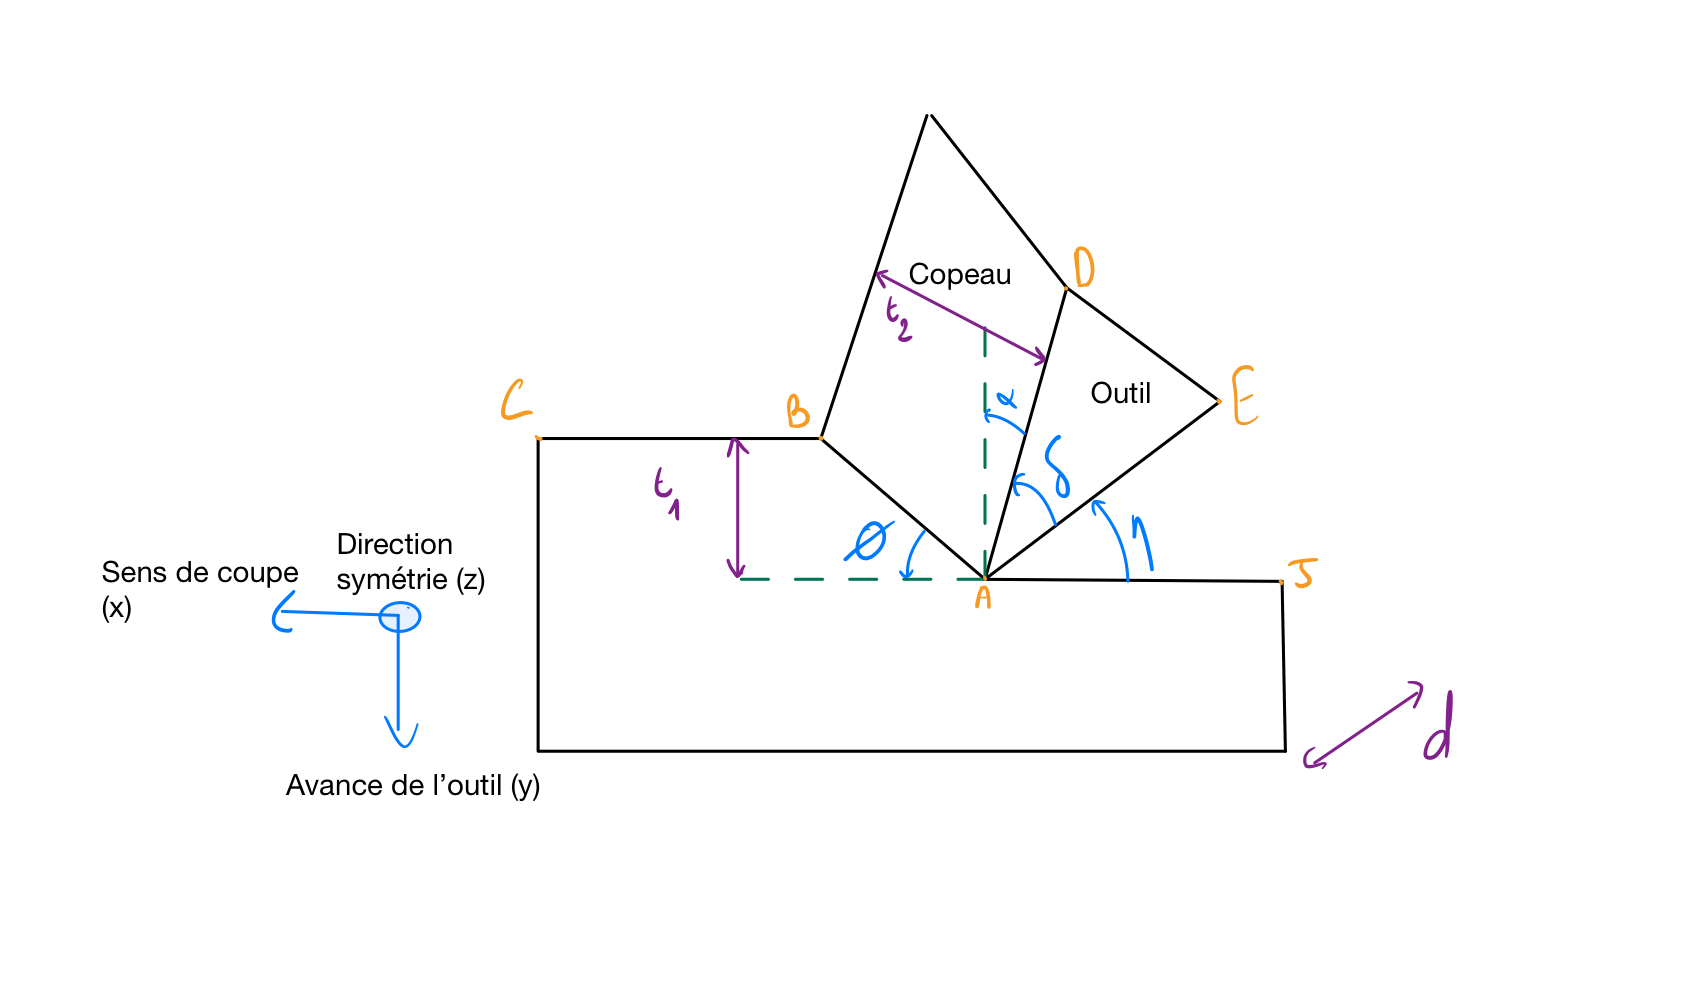
\includegraphics[width=.8\textwidth]{IMAGES/procprod/coupeortho.png}
\end{figure}

\begin{minipage}{.5\textwidth}
    \begin{itemize}
        \item $t_1$ : épaisseur couche cisaillement\\
        \item $t_2$ : épaisseur copeau\\
        \item $d$ : profondeur coupe\\
        \item $\alpha$ : angle de coupe\\
        \item $\delta$ : angle tranchant\\
        \item $\eta$ : angle de dépouille\\
        \item $\phi$ : angle de cisaillement\\
    \end{itemize}
\end{minipage}
\begin{minipage}{.5\textwidth}
    \begin{itemize}
        \item AD : surface de coupe\\
        \item AE : surface de dépouille\\
        \item BC : surface à usiner\\
        \item AJ : surface usinée\\
        \item AB : plan de cisaillement\\
        \item A : arête de coupe\\
    \end{itemize}
\end{minipage}

On a : $\eta + \delta + \alpha = \frac{\pi}{2}$ et $-\frac{\pi}{2}<\alpha<\frac{\pi}{2}$, $0<\phi< \min(\frac{\pi}{2}, \frac{\pi}{2}+\alpha)$\\

\textbf{Rapport de coupe :} $R = \frac{t_1}{t_2} = \frac{\sin{\phi}}{\cos(\phi-\alpha)}$\\
Avec : $t_1 = \lVert AB\rVert \sin{\phi}$ et $t_2 = \lVert AB\rVert \cos{\theta}$ où $\theta = \phi-\alpha$\\

On a donc : $\gamma = \frac{1}{2}(\cot{\phi} + \tan(\phi - \alpha))$\\

A angle $\alpha$ fixé, le taux de cisaillement est minimum pour $\phi = \frac{\pi}{4} + \frac{\alpha}{2}$\\
Il vaut donc : $\gamma_{min} = \tan(\frac{\pi}{4} + \frac{\alpha}{2}) \Rightarrow \gamma_{min}(\alpha) = \begin{cases}
    0 & \text{si}\quad \alpha \rightarrow \frac{\pi}{2}\\
    \infty & \text{si}\quad \alpha \rightarrow -\frac{\pi}{2}\\
\end{cases}$

\subsubsection{Cinématique de la coupe}
\begin{itemize}
    \item vitesse de coupe : déplacement de la lame $v$\\
    \item déplacement de la partie coupée (copeau) : $v_s = \frac{\cos{\alpha}}{\cos(\phi-\alpha)}v$\\
    \item déplacement de la base du copeau : vitesse de frottement $v_f = \frac{\sin{\phi}}{\cos(\phi-\alpha)}v$\\
    \item volume de matière coupée : $\dot{V}_c = vt_1 d $ MRR (material removal rate)\\
    \item volume de matière dans le copeau : $\dot{V}_{cop} = v_f t_2 d$\\
    \item taux de dilatation du copeau : $a_{dil} = \frac{\dot{V}_{cop}}{\dot{V}_c}-1$\\
\end{itemize}

On peut décomposer la force émise sur la matière comme une composante de coupe : $F_c = F \cos(\alpha-\beta)$ et une force d'avance : $F_{av} = F\sin(\alpha-\beta)$, avec $\tan{\beta} = \mu$ et $0<\beta<\frac{\pi}{2}$\\

\subsubsection{Théorie de Merchant}
La coupe ne peut avoir lieu que si la force exercée par la lame sur le copeau est dirigée dans la direction de coupe : $F_c>0 \Rightarrow \cos(\alpha-\beta) >0 \Rightarrow -\frac{\pi}{2}<\alpha-\beta<\frac{\pi}{2}$\\

La force globale exercée peut se décomposer en plusieurs éléments. Premièrement en une force de frottement agissant sur l'objet :\\
\begin{equation}
    F_f = F \sin{\beta}
\end{equation}

Dès lors, la force exerce cisaillement sur le matériaux : \\
\begin{equation}
    F_s = F\cos(\phi-(\alpha-\beta))
\end{equation}
Celle ci applique une contrainte de cisaillement $\tau$ avec pour aire de la surface de cisaillement $A_s = \frac{dt_1}{\sin{\phi}}$. \\

\begin{equation}
    \tau(\phi) = \frac{F_s}{A_s} = \frac{F}{dt_1} \sin{\phi} \cos(\phi-(\alpha-\beta)) = \frac{F_c}{dt_1 \cos(\alpha-\beta)}\sin{\phi} \cos(\phi-(\alpha-\beta))
\end{equation}

On veut donc choisir $\phi$ tel qu'il maximise $\tau$ et minimise $F_c$. Le matériaux se fend sous l'angle de cisaillement si la contrainte appliquée atteint le niveau de résistance au cisaillement $\tau_s$ du plan incliné $\tau(\phi) = \tau_s(\phi)$. On a donc :\\
\begin{equation}
    F_c = F_c(\phi) = \frac{\tau_s(\phi)}{\sin{\phi} \cos(\phi-(\alpha-\beta))}dt_1 \cos(\alpha-\beta)
\end{equation}
Pour un matériaux anisotrope, on peut donc trouver que : \\
\begin{equation}
    \phi_{M;gen} = \arg \min_{\phi\in (0, \min\{\frac{\pi}{2}, \frac{\pi}{2}+(\alpha-\beta)\})} F_c(\phi)
\end{equation}

Pour un matériaux isotrope, on a que $\tau_s(\phi) = \tau_s$. On a donc :\\
\begin{equation}
    \phi_M = \frac{\pi}{4}+\frac{\alpha-\beta}{2}
\end{equation}

Pour que le matériaux se coupe, il faut que $\max \tau = \frac{F_c}{2dt_1 \tan(\frac{\pi}{4}-\frac{\alpha-\beta}{2})} = \tau_s$. Ainsi la force de coupe doit valoir :\\
\begin{equation}
    F_c = 2\tan(\frac{\pi}{4}-\frac{\alpha-\beta}{2}) \tau_s dt_1
\end{equation}

On définit alors la \textbf{puissance de coupe} : \\
\begin{equation}
    P_c = F_cv = 2\tan(\frac{\pi}{4}-\frac{\alpha-\beta}{2})\tau_s vdt_1 = e_c vdt_1
\end{equation}
Avec $e_c$ l'énergie spécifique de coupe : $e_c = \frac{P_c}{\dot{V}_c}$. \\
On peut décomposer la puissance de coupe en deux composantes : la puissance de cisaillement et de frottement : \\
\begin{equation}
\begin{gathered}
    P_c = P_f+P_s\\
    P_f = F_fv_f = 2\tau_s \frac{\sin{\beta}}{\cos{\beta}+\sin{\alpha}} vdt_1\\
    P_s = F_sv_s = 2\tau \frac{\cos{\alpha}}{\cos{\beta}+\sin{\alpha}} vdt_1
    \end{gathered}
\end{equation}

La puissance de coupe est presque entièrement dissipée sous forme de chaleur ($E_{elas}<0.02 E_{tot}$)\\

On a les différentes valeurs :\begin{itemize}
    \item chaleur apportée au copeau : $\dot{Q}_c = \eta_c P_c = \eta_c e_c vt_1d$ [W] ($\eta_c \simeq 75\%$)\\
    \item chaleur apportée à l'outil : $\dot{Q}_o = \eta_o P_c = \eta_o e_c vdt_1$[W] ($\eta_o \simeq 20\%$)\\
    \item chaleur apportée à la pièce : $\dot{Q}_p = \eta_p P_c = \eta_p e_c vdt_1$[W] ($\eta_p \simeq 5\%$)\\
\end{itemize}
Si on fait de l'usinage à grande vitesse (ugv), presque toute l'énergie est transférée au copeau.\\
L'énergie spécifique de coupe ($e_c$ [J/$m^3$]) vaut $e_c = \frac{P_c}{\dot{V}} = \frac{F_c}{td_1}$\\
La moyenne temporelle vaut $\overline{P} = e_c \dot{\overline{V}}$ avec $\dot{\overline{V}} = \frac{V_c}{T}$, T la durée de l'opération.\\


\subsubsection{Analyse thermique de l'outil}
On considère une température stationnaire en un point de l'outil. La fonction de température est harmonique, on a donc $\frac{\partial^2 T}{\partial x^2} + \frac{\partial^2T}{\partial y^2} = 0$ dans l'outil. \\

On a aussi les conditions : $\begin{cases}
    T = 0 & \text{sur arête opposée DE}\\
    \partial_n T = \frac{\dot{Q}_o}{\lambda d}\kappa  = \frac{\eta_o e_c vt_1}{\lambda}\kappa& \text{sur les deux arêtes adjacentes AD}\cup \text{AE}\\
\end{cases}$

On a donc $T(x,y) = \frac{\eta_o e_c vt_1}{\lambda} \theta(x,y)$, avec $\begin{cases}
    \theta = 0 & \text{sur DE}\\
    \partial_n \theta = \kappa & \text{sur AD}\cup \text{AE}
\end{cases}$
On admet aussi que $\kappa(x) = \frac{1}{\parallel AD\parallel +\parallel AE\parallel}$\\

Ainsi, pour diminuer l'échauffement, on peut augmenter la conductivité thermique, diminuer la vitesse ou l'épaisseur de la pièce, diminuer l'énergie spécifique de coupe voire diminuer $\eta_0$ par lubrification.\\

\subsubsection{Usinabilité des matériaux}
\quad \underline{Définition :} l'usinabilité d'un matériaux est son aptitude à être usiné par enlèvement de copeaux.\\

L'indice d'usinabilité est une façon de résumer les données empiriques des expériences de coupe. C'est une mesure de : \begin{itemize}
    \item état de surface atteignable\\
    \item durée de vie outile\\
    \item vitesse de coupe\\
    \item force de coupe
\end{itemize}
\color{gray}Note : une usinabilité de 100\% correspond à une durée de vie de l'outil (HSS) de 60min à 100ft/min avec des conditions de coupe standard. \color{black}\\

L'usinabilité est influencée par le type de matériaux ainsi que par sa micro-structure.\\

\subsubsection{Usure des outils}
Plusieurs causes : \begin{itemize}
    \item usure par adhésion : arête rapportée sur la face de coupe\\
    \item usure par abrasion : frottement sur la face de dépouille\\
    \item usure par diffusion : migration des atomes\\
\end{itemize}

On utilise un modèle empirique pour décrire les effets de l'usure sur la face de dépouille.\\
\quad \textbf{Modèle de Taylor} : \\
\begin{equation}
    vLT^n d^x t_1^y = C
\end{equation}
Avec $v$ la vitesse de coupe, $LT$ la durée de vie, d la profondeur de coupe et $t_1$ l'épaisseur de coupe.\\
x,y et C sont déterminés expérimentalement.\\
\begin{table}[hbt!]
    \centering
    \begin{tabular}{c|c}
        \hline
        High-speed steel & 0.08-0.2  \\
        Carbides & 0.2-0.5\\
        Ceramics & 0.5-0.7\\
        \hline
    \end{tabular}
    \caption{n typiques}
\end{table}


\subsubsection{Familles principales de matériaux}
\begin{itemize}
    \item \underline{Aciers rapides (HSS)} :\begin{itemize}
        \item Aciers outils fortement alliés conservant leur propriété de trempe même à haute température, par coulée puis forgeage\\
        \item Avantages : faible coût, haute tenaité, facilité de mise en forme\\
        \item  Désavantages : dureté limitée, résistance à l'usure limitée\\
        \item Applications : angle de coupe élevé, faible vitesse de coupe (acier 25-40m/min, alu 50-100m/min)\\
    \end{itemize}
        \item \underline{Carbures métalliques} :\begin{itemize}
        \item par frittage\\
        \item Avantages : dureté à chaud et E plus élevé que HSS, bon k, coefficient de dilatation plus faible que HSS\\
        \item  Désavantages : ténacité moins bonne que HSS, coût supérieur à HSS\\
        \item Applications : usinage des aciers, fontes et alliages non ferreux abrasifs, alliages légers, vitesse de coupe (acier 100-200m/min, alu 1000-3000m/min)\\
    \end{itemize}
        \item \underline{Outils revêtus} :\begin{itemize}
        \item base = HSS, carbures métalliques, revêtement mono-multicouches\\
        \item Avantages : dureté à chaud élevée, faible coefficient de friction, bonne stabilité chimique, durée de vie plus longue\\
        \item  Désavantages : coût élevé, tendance à la dé-cohésion du revêtement\\
        \item Applications : usinage similaire aux carbures métalliques, vitesses de coupe plus grande que le matériaux de base\\
    \end{itemize}
            \item \underline{Céramiques} :\begin{itemize}
        \item Avantages : dureté à chaud élevée, haute résistance à l'abrasion, bonne stabilité chimique\\
        \item  Désavantages : fragile, faible ténacité, sensibles aux chocs thermiques\\
        \item Applications : vitesses de coupe élevées, machine haute rigidité, usinage de finition des aciers et fontes\\
    \end{itemize}
            \item \underline{Nitrures de bore cubiques} :\begin{itemize}
        \item Avantages : Très haute dureté, haute résistance à l'usure\\
        \item  Désavantages : fragile, faible ténacité, sensibles aux chocs et vibrations\\
        \item Applications : usinage des aciers trempés et alliages réfractaires, machines et bridage à haute rigidité\\
    \end{itemize}
            \item \underline{Diamant} :\begin{itemize}
        \item Avantages : dureté extrême, résistance à l'usure, faible coefficient de friction, haute conductivité thermique\\
        \item  Désavantages : décomposition si $T>700^\circ C$, faible ténacité, fragile, sensible aux chocs, coût élevé\\
        \item Applications : opération de finition sur matériaux non-ferreux, usinage très haute précision\\
    \end{itemize}
\end{itemize}



\subsection{Fonderie}
Procédé de production de pièces métalliques réplicatif. Mise en forme dans un moule de fonderie.\\

\underline{Atouts :} \begin{itemize}
    \item possibilité de fabriquer des pièces complexes\\
    \item pièces de plusieurs grammes jusqu'à plusieurs tonnes\\
    \item valable pour beaucoup d'alliages dur à usiner\\
    \item pour des petites à grandes séries\\
\end{itemize}

\underline{Généralement :} moules de fonderie sont en \begin{itemize}
    \item en sable : non permanent (1pièce) \begin{itemize}
        \item en sable\\
        \item en cire perdue : valable de 1g à 10kg, bon état de surface, moule perdu, on entoure la cire avec de la céramique pour faire une carapace, ensuite on chauffe jusqu'à la température du métal pour éviter le choc thermique\\
        \item en carapace : \begin{itemize}
            \item moule de sable à durcissement chimique à chaud\\
            \item plaque modèle chauffée entre 200 et 300$^\circ$\\
            \item sable aggloméré sur la plaque par fusion de la résine\\
            \item chaîne de procédé duplicative à modèle maître\\
            \item Avantages : valide pour tous les matériaux de fonderie, fabrication de 50 à 60 carapace par heure, bon état de surface\\
            \item Inconvénients : outillage coûteux\\
        \end{itemize}
        \item en motte  :\begin{itemize}
            \item sable pressé à plus de 10bar, pas de châssis, les moules doivent se suivre\\
            \item Avantages : bonne précision, 240 moules/heure\\
            \item Inconvénients : pose de noyau compliqué\\
        \end{itemize}
    \end{itemize}
    
    \item en métal : permanent (N pièces) \begin{itemize}
        \item par gravité \\
        \item basse pression\\
        \item haute pression (chambre froide voire chaude)\\
        \item centrifuge\\
    \end{itemize}
\end{itemize}

\subsubsection{Non-permanents}
\underline{En sable :} fabriqué à la main à partir de sable que l'on serre dans un châssis\\
Chaîne de procédés \textbf{duplicative}.\\
Modèle est appelé \textbf{modèle maître} s'il est réutilisable et \textbf{modèle perdu} s'il faut le casser. Le moule est fabriqué par procédé réplicatif.\\
Le moule est obtenu après retrait du modèle via \textbf{démoulage}. On a appelle le plan de séparation des parties du moule les \textbf{plans de joints}.\\
\warning règles (paroi fines, épaisseur = constante, pas d'angle droit)\\

La pose de \textbf{noyau} à l'intérieur de l'empreinte est nécessaire si la pièce à réaliser est creuse.\\
L'empreinte est remplie de métal en fusion par \textbf{trou de coulée}. \\
La pièce est récupérée après destruction du moule par \textbf{décochage}. Le moule est un outil de formage \textbf{sacrificiel}. \\
La \textbf{masselotte} est là pour compenser les défauts de fonderie comme les retassures.\\

\begin{minipage}{.5\textwidth}
    \underline{3 volumes :} $V_p$ : pièces\\
    $V_m$ : masselotte\\
    $V_{tc}$ : trou de coulée\\
\end{minipage}
\begin{minipage}{.5\textwidth}
    mise en mille $= \frac{V_p + V_m + V_{tc}}{V_p}$
\end{minipage}

Il existe plusieurs types de modèles :\\
\begin{itemize}
    \item solide : copie exacte de la pièce\\
    \item séparés : la pièce est séparée en deux parties\\
    \item plaques de joints (entière avec plaque au milieu)\\
    \item poinçon-matrice (avec trou de coulée et masselotte)\\
\end{itemize}

Le noyau est composé d'une forme (dans le vide) et d'une guirlande (support)\\

Qualité du sable \begin{enumerate}
    \item résistance : garder sa forme/résister à l'érosion\\
    \item perméabilité : évacuer l'air et les gaz\\
    \item stabilité thermique : faculté de la cavité à résister aux fissures lors de l'arrivée du métal liquide\\
    \item compliance : faculté du moule à laisser le métal se retirer sans craquer\\
    \item décochabilité : facilité à éliminer le sable de la pièce coulée\\
    \item réutilisabilité : recyclage du sable\\
\end{enumerate}

Aujourd'hui, on fabrique les moules via des procédés additifs. Dans ce cas, le moulage en sable ne conduit plus une chaîne de procédés duplicative.\\

On distingue deux types de sables \begin{enumerate}
    \item non durcis/sables à vert voire naturels, plusieurs possibilités : \begin{itemize}
        \item on peut sécher par étuvage : \textbf{moule étuvés}\\
        \item ou on peut sécher la surface du moule (air chaud, flamme, $\dots$) : \textbf{moule flambées}\\
    \end{itemize}
    \item sables à durcissement chimique (mélange silice, argile, $\dots$, et un adjuvant), durcissement à chaud et à froid\\
\end{enumerate}
Il existe 4 types d'adjuvants :\begin{itemize}
    \item ciment (à froid)\\
    \item silicate de soude (à froid) : tendance à s'effriter, recyclable\\
    \item résine furaniques/phénoliques (à chaud) : durcissement par catalyseur\\
    \item résines thermodurcissables (à chaud) : durcissement à plus de 200$^\circ$C\\
\end{itemize}

\quad \underline{Gamme d'opération :}\\
\begin{itemize}
    \item moulage : fabrication du modèle\\
    \item démoulage : enlèvement du modèle\\
    \item noyautage : fabrication des noyaux\\
    \item remoulage : préparation du moule (assemblage des parties)\\
    \item fusion : obtention du métal liquide\\
    \item coulée : remplissage du moule\\
    \item décochage : ouverture du moule\\
    \item débourrage : destruction du noyau\\
    \item ébarbage et finition : tronçonnage du jet de coulée, meulage\\
    \item opérations secondaires : traitement thermique\\
\end{itemize}

\subsubsection{Moules permanents}
Moules en métal plutôt que sable.\\
Les moules sont donc réutilisable, refroidissement plus rapide. Limitation aux métaux à faible point de fusion.\\

Plusieurs méthodes :\\
\begin{itemize}
    \item Moulage par gravité : préchauffage requis pour éviter les choc thermique. Le liquide coule dans le moule par gravité. Durée de vie sans retouche est d'environ 500pièces.\\
    \item Basse pression : liquide sous le moule et poussé dedans via gaz sous pression. Le trou de coulée est beaucoup moins grand.\\
    \item Haute pression : métal injecté dans le moule par un piston qui se déplace dans une chambre (la pression peut atteindre 1000bar). Le moule est formé de deux blocs. On peut avoir une \textbf{chambre froide} qui est alimentée en métal fondu par une trémie, il y a ici un risque de blocage de la chambre si le métal se refroidit trop vite. Il y a aussi la \textbf{chambre chaude} qui évite ce problème.\\
    \item Centrifuge : moule en rotation autour d'un axe. La coulée est dans la direction de l'axe de rotation. Avantages : bon contrôle de la solidification, on obtient les meilleures propriétés possible par un procédés de production, influence sur la micro-structure avec le débit de coulée. Inconvénients : pas de noyau possible\\
\end{itemize}

\quad \underline{Défauts de fonderie :}\\
\begin{itemize}
    \item Malvenue : la zone manquante qui apparaît lorsque le métal se solidifie complètement avant d'avoir atteint entièrement le bord de la cavité\\
    \item Goutte froide : défaut interne qui apparaît à l'endroit où deux flux opposés de métal liquide n'ont pas réussi à s'unir avant solidification. \textbf{Causes :} mauvaise fluidité du métal, température de coulée trop basse\\
    \item Retassures : dépression externe. Elles sont reliées au retrait de solidification qui peut réduire la quantité de matériaux dans la dernière région qui se solidifie. \textbf{Solution :} adaptation du masselottage, contrôle de la pression\\
    \item Criques : défauts apparaissent lorsque la trop grande rigidité du moule empêche le retrait naturel de la pièce : fissure aux endroits de tension. \textbf{Solutions : } Amélioration de la collapsibilité du sable, éjection rapide de la pièce\\
    \item Piqûres et soufflures : il y a des gaz dissous dans le métal et dégagent pendant la solidification, ce qui crée des petites cavités (piqûres $\phi<2mm$). Le mouvement de coulée peut faire percoler du gaz depuis les moules en sables, on a des cavités plus grandes : soufflures $\phi<1cm$\\
    \item Macroségrégation : lié à la coulée d'alliages. Les mouvements de convection créent des inhonomogéneité de $c_{solute}$ à l'échelle macroscopique. Il y a donc une perte des propriétés mécaniques. \textbf{Cause :} écoulement forcé lié à la coulée, retrait de solidification, force d'archimède. \textbf{Solutions :} contrôle des mouvements par application de force extérieures.\\
\end{itemize}

Il existe trois grand types de problèmes liés à la fonderie en sable :\\
\begin{itemize}
    \item interaction physico-chimique entre moule et la pièce : \begin{itemize}
        \item marbrures : tâches sur la pièces (incrustation du sable dans le métal)\\
        \item pénétration : infiltration du métal dans le sable\\
    \end{itemize}
    \item dommages provoqués sur le moule par le métal : \begin{itemize}
        \item érosion pendant la coulée\\
        \item fissuration dans les moules résistants\\
    \end{itemize}
    \item déplacement relatif du moule :\begin{itemize}
        \item décalage des noyaux\\
        \item décalage des parties supérieures et inférieures\\
    \end{itemize}
\end{itemize}

\subsubsection{Matériaux de fonderie}
\quad \underline{Fontes :}\\
Alliages de fer riches de 2.1\% à 6.8\% de carbone. Coulabilité excellente, température de fusion entre 1141$^\circ$ et 1350$^\circ$. Le métal cristallise soit avec de la ferrite et de la graphite (fonte grise), soit avec de la ferrite et de la cémentite (fonte blanche, méta-stable).\\

La fonte grise est favorisé par l'addition de silicium ainsi que des vitesses de solidification faibles. Alors que la fonte blanche est favorisé par de faible teneur en carbone et silicium et par des vitesses de solidification élevées.\\
\underline{Fonte blanche :} bonne coulabilité, très résistant à l'usure et à l'abrasion. Cependant, usinabilité délicate.\\
\underline{Fonte grise :} excellente coulabilité, pas cher, absorption des vibrations, résistant à la corrosion et déformable à chaud. Cependant, elle est fragile comparé aux acier et fontes blanches.\\

\quad \underline{Alliages cuivre :} principalement du bronze (Cu-Sn). Le laiton (Cu-Zn) est moins courant.\\
Il sont résistant à la corrosion et à l'usure. Cependant il sont cher.\\

\quad \underline{Aluminium :} un des meilleurs matériaux pour la fonderie. Il est léger, a une bonne usinabilité et peut former une grande gamme de résistance. Sa température de coulée est basse : $T_m = 660^\circ C$.\\

\quad \underline{Alliages zinc :} le zinc et ses alliages sont utilisés en injection métallique. Il a une très bonne coulabilité et une température de coulée très basse : $T_m = 419^\circ C$.\\"

\subsubsection{Principe physique de la fonderie}
\quad \underline{Analyse thermique de la fonderie :}\\
\underline{Hypothèses de Chvorinov :} il existe un profil de refroidissement analytique valable au voisinage de l'interface moule/cavité. On a les hypothèses :\begin{itemize}
    \item l'interface est le plan $x=0$, moule dans le domaine $x<0$, pièce dans le domaine $x>0$\\
    \item $T=T(t,x)$\\
    \item $\rho, c_T,k$ sont constants\\
    \item le métal est un corps pur et il possède les mêmes propriétés en liquide que solide\\
\end{itemize}

Soit $\beta>0$ (sans unité) et $T_i$ la température d'interface moule/métal\\
La position du front solide/liquide est donnée par $x_{sl}(t) = 2\beta \sqrt{\eta t}$, la vitesse d'avance du front est donnée par : $v_{sl}(t) = \frac{\eta \beta}{\sqrt{\eta t}}$\\

\begin{equation}
    T(t,x) = \begin{cases}
        T_i + (T_i-T_m) erf(\frac{x}{2\sqrt{\eta_m t}}) & -\infty<x<\infty\\
        T_i + \frac{T_f-T_i}{erf(\beta)}erf(\frac{x}{2\sqrt{\eta t}}) & 0\leq x\leq x_{sl}\\
        \frac{T_f-T_c erf(\beta)}{1-erf(\beta)}+\frac{T_c-T_f}{1-erf(\beta)}erf(\frac{x}{2\sqrt{\eta t}}) &x_{sl} \leq x \leq \infty\\
    \end{cases}
\end{equation}

\color{gray} Fonction erreur : primitive de erf'$(t) = \frac{2}{\sqrt{\pi}}e^{-t^2}$ avec erf$(0) = 0$, erf$(\pm \infty) = \pm 1$. Elle satisfait $\partial_t erf(\frac{x}{2\sqrt{t}}) = \partial_{xx} erf(\frac{x}{2\sqrt{t}})$ \color{black}\\

On a dès lors :\begin{equation}
    \partial_x T(t,x) = \begin{cases}
        \frac{T_1-T_m}{\sqrt{\pi \eta_m t}} e^{-\frac{x^2}{4\eta_m t}} & -\infty < x \leq 0\\
        \frac{T_f-T_i}{\sqrt{\pi \eta t} erf(\beta)} e^{-\frac{x^2}{4\eta t}} & 0\leq x \leq x_{sl}(t)\\
        \frac{T_c-T_f}{\sqrt{\pi \eta t}(1-erf(\beta))}e^{-\frac{x^2}{4\eta t}} & x>x_{sl}\\
    \end{cases}
\end{equation}

On a $T_i$ la température d'interface moule/cavité, elle est constante dans le temps.\\
A cette interface, on a $\Delta x \simeq 0$ à $x=0$\\
On a $\dot{q}_{\text{sortant du moule}} = -k_m \partial_x T_{\rvert x=0^-}$ et $\dot{q}_{\text{sortant de la cavité}} = k\partial_x T_{\rvert x=0^+}$ \\
Soit pour bilan : $\dot{q}_{\text{sortant du moule}} + \dot{q}_{\text{sortant de la cavité}} = -k_m (T_i-T_m) + k(T_f-T_i)$\\

\begin{equation}
\begin{gathered}
    T_i = w_mT_m+w_fT_f\\
    \begin{cases}
        w_m = \frac{erf(\beta)}{erf(\beta)+\xi}\\
        w_f = \frac{\xi}{erf(\beta)+\xi}\\
    \end{cases}\\
    \xi = \frac{k \sqrt{\eta_m}}{k_m \sqrt{\eta}}\\
    \eta = \frac{k}{\rho C_p}
\end{gathered}
\end{equation}

A l'interface solide/liquide ($x=x_{sl}(t)$)\\
A temps t, on a du liquide à $T_f$\\
A temps $t+\Delta t$ on a du solide à $T_f$\\

\begin{itemize}
    \item Masse : $\rho S v_{sl}(t) \Delta t$\\
    \item avant : $\rho S  v_{sl}(t) \Delta t u_{av} = \rho S v_{sl}(t) \Delta t(C_pT_f+L)$\\
    \item après : $\rho S v_{sl}(t) \Delta t u_{ap} = \rho S v_{sl}(t) \Delta t C_pT_f$\\
    \item entrant de gauche : $S \phi_g \cdot \hat{n}_g \Delta t = -kS \partial_x T_{\lvert x_{sl}-}\Delta t$\\
    \item entrant de droite : $S\phi_d \cdot \hat{n}_d \Delta t = k S \partial_x T_{\lvert x_{sl}+} \Delta t$\\
\end{itemize}
$\Rightarrow \rho S v_{sl} \Delta t C_p T_f = \rho S v_{sl} \Delta t (C_p T_f+L)-kS \partial_x T_{\lvert x_{sl}-} \Delta t + kS \partial_x T_{\lvert x_{sl}+}\Delta t$\\

\begin{equation}
    \begin{gathered}
        k \partial_x T_{\lvert x_{sl}-} - k \partial_x T_{\lvert x_{sl}+} = \rho L \frac{\eta \beta}{\sqrt{\eta t}}\\
        \sqrt{\pi} L \beta e^{\beta^2} = \frac{C_p (T_f-T_m)}{erf(\beta)+\xi} + \frac{C_p(T_c-T_f)}{erf(\beta)-1}
    \end{gathered}
\end{equation}

\color{gray} Note : existence d'une solution si et seulement si le membre de droite est positif lorsque $\beta = 0$ $\Rightarrow T_f-T_m > \xi(T_c-T_f)$.\\
Le membre de droite est décroissante et le membre de gauche est croissante.\\

En général $T_c \simeq T_f \Rightarrow \sqrt{\pi}L\beta e^{\beta^2} \simeq \frac{C_p(T_f-T_m)}{erf(\beta)-\xi} \Rightarrow \sqrt{\pi} \beta e^{\beta^2} (\xi +erf(\beta)) = \frac{C_p(T_f-T_m)}{L}$ si on a $<<1$ alors on peut approximer $\beta$ avec $\hat{\beta} = \frac{C_p(T_f-T_m)}{\sqrt{\pi}L\xi}$ car $e^{\beta^2}\simeq 1$ et $erf(\beta)\simeq 0$\\
\color{black}\\

\quad \underline{Calcul du temps $t^*$ pour solidifier un volume $V^*$ :}\\
Soit A : aire interface moule/cavité tel que $Ax_{sl}(t^*) = V^* = 2\beta A \sqrt{\eta t^*} \Rightarrow t^* = (\frac{V^*}{2\beta A})^2 \frac{1}{\eta}$\\

Pour des pièces à toute géométries : $t^* = B (\frac{V}{A})^n$, n généralement 2, A aire latérale et B un coefficient qui ne dépend que des propriétés thermiques du moule/métal\\

Il existe deux types de solidification : \begin{itemize}
    \item solidification en \textbf{front plan} : (pour mono-cristallin) si fraction liquide passe de 0 à 1 au travers d'une surface appelée front de solidification\\
    \item solidification en \textbf{zone pâteuse} si fraction liquide passe continûment de 0 à 1 au travers d'un domaine appelée zone pâteuse\\
\end{itemize}

\quad \underline{Critère de stabilité du front plan ($c^* < c_{max}$) :}\\

Pendant la solidification, un mécanisme physique déstabilise les fronts plans : formation d'une zone \textbf{de surfusion} due à : \begin{itemize}
    \item la décroissance de la concentration de soluté dans le liquide devant le front\\
    \item l'augmentation de la température de liquidus lorsque la concentration de soluté diminue\\
\end{itemize}

La condition d'instabilité est liée au gradient G de la température imposée :\begin{equation}
    -m\partial_x c_{\lvert \text{av .front}}>G = \partial_x T_{\lvert \text{av. front}}
\end{equation}

\quad \underline{Calcul de $\partial_x c_{\lvert \text{av. front}}$ :}\\
La masse de soluté quitte le front par udt : $\dot{M} = S \Vec{q}\cdot \hat{n} = -SD \partial_x c_{\lvert \text{av. front}}$\\

\textbf{Loi de diffusion :} $\Vec{q} = -D \text{grad} c$ g/s/mm$^2$\\

\begin{equation}
    -\partial_x c_{\lvert \text{av. front}} = \frac{\rho v_{sl}}{D} c^*(\frac{1}{k}-1)
\end{equation}

\quad \underline{Zone pâteuse :}\\
Si le rapport $\frac{G}{v_{sl}}$ est petit, le front plan est déstabilisé par des \textbf{dendrites} ou \textbf{grains équiaxes} dans la zone pâteuse.\\

\underline{Critère de Hunt :} $v_{sl}$ favorise les dendrites lorsque qu'elle est élevée. Si G est petit, on trouvera alors plus de grains équiaxes.\\

\underline{Joints de grains :} intersection entre les dendrites et les grains demeurent visibles après la coulée sous forme de joints de grains.\\

Dans la zone pâteuse, la concentration en soluté reste constante : la richesse du liquide en soluté est compensée par la création locale de solide pauvre en soluté (micro-ségrégation)\\

\quad \underline{Pas de diffusion dans soluté :}\\

On a $kc^*<c<c_{max}$ et la fraction eutectique (de même pour la fraction liquide) : $f_L^E = \sqrt[1-k]{\frac{c^*}{c_E}}$, $f_\alpha = \frac{c'_{max}-c_E}{c'_{max}-c_{max}}$ et $f_\beta = \frac{c_E-c_{max}}{c'_{max}-c_{max}}$\\
\warning A l'interface solide zone pâteuse, on a $f_L = 0$ ce qui est impossible s'il n'y a pas de diffusion, on a donc $T = T_e$ la température eutectique. De plus, il apparaît un palier de fusion qui se trouve à la température $T_e$, où la fraction de liquide eutectique du côté solide-palier vaut 0 et de l'autre côté $f_L$ donnée par la formule de Scheil. Si la diffusion est supposée infinie, alors $c_s = c^*$ et $T = T_s = T_f- \frac{m}{k}c^*$. \\
\warning $c_L = \frac{c_s}{k}$

\begin{figure}
    \centering
    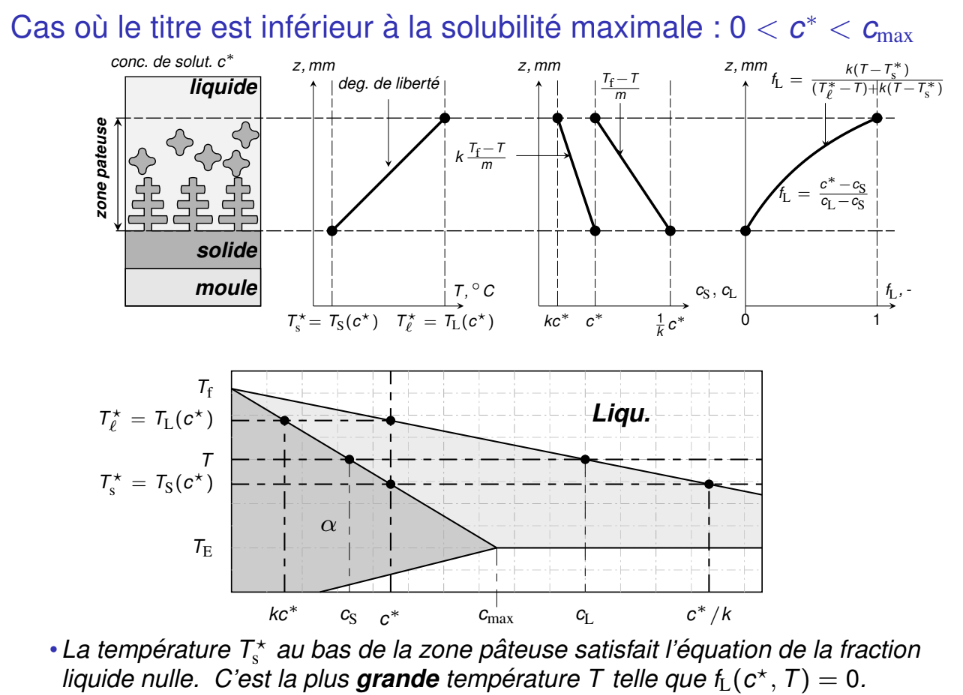
\includegraphics[width=\textwidth]{IMAGES/procprod/proc62.png}
    \caption{$c<c_{max}$}
\end{figure}

\begin{figure}
    \centering
    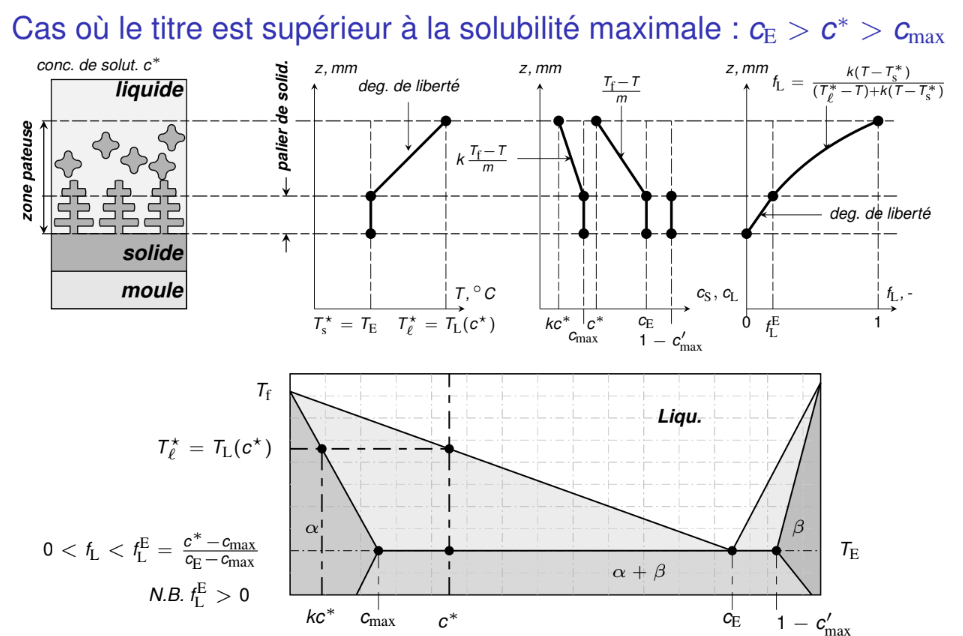
\includegraphics[width=\textwidth]{IMAGES/procprod/proc61.png}
    \caption{$c>c_{max}$}
\end{figure}

\quad \underline{Déplacement du fluide :}\\
Soit $V_A$ la vitesse de coulée\\
\underline{Hypothèses :} écoulement non visqueux, incompressible et laminaire\\
\underline{Équations de continuité :} $S_Av_A = S_Bv_B = \dots \Rightarrow \frac{1}{2}\rho v_A^2+\rho g h_A + P_A = C$\\
\warning Non valable à travers une expansion; on la remplace par $P_E \simeq P_E'$\\

\subsection{Formage}
On utilise la déformation plastique pour mettre en forme. On a donc un procédé réplicatif.\\
L'outil de forme est ici une matrice et un poinçon.\\

La formabilité est favorisé par une grande ductilité et une faible limite élastique.\\

\underline{Avantages :} pièces complexes possibles, valable pour beaucoup de métaux et uniquement pour grandes voire très grandes séries.\\

\subsubsection{Forgeage}
Compression de la pièce dans une matrice. Le forgeage à froid admet de meilleures propriétés mécaniques et est plus précis. \\
\begin{table}[hbt!]
    \centering
    \begin{tabular}{c|c}
    \hline
        compression par impact & compression graduelle \\
        martelage & pressage\\
        forgeage libre & matriçage (via poinçon)\\
        \hline
    \end{tabular}
    \caption{Types de forgeages}
\end{table}

\quad \underline{Force en forgeage libre :} $\varepsilon = \ln(\frac{h_0}{h})$ et $F_f^0 = S_f k (\ln(\frac{h_0}{h_f}))^n = S_f \sigma_e = S_0 R_e$ (comportement idéalement plastique).\\
Valable si pas de frottements.\\

Si on prend en compte les frottements, alors l'objet risque la mise en tonneau.\\
On a alors : $F_f^\mu = (1+C\mu \frac{\sqrt{S_f}}{h_f}) F_f^0$, avec C un coefficient dépendant de la géométrie de la pièce ($C\simeq 0.45$ section circulaire)\\

\quad \underline{Matriçage de précision :} le matériaux ne s'écoule pas en dehors de la matrice (pas de bavure)\\

\subsubsection{Laminage}
On effectue ici une réduction de l'épaisseur en comprimant le matériaux entre deux rouleaux. En général, on le fait à chaud pour limiter les contraintes internes.\\

\begin{table}[hbt!]
    \centering
    \begin{tabular}{c|c}
        \hline
        vitesse angulaire rouleaux & $\omega_d$ \\
        rayon rouleaux & R\\
        vitesse rouleaux & $v_d$\\
        angle de contact & $\theta$\\
        longueur de contact & L\\
        vitesse entrée & $v_0$\\
        vitesse sortie & $v_f$\\
        épaisseur/largeur entrée & $t_0,w_0$\\
        épaisseur/largeur sortie & $t_f,w_f$\\
    \end{tabular}
    \caption{Variables}
\end{table}

On a par ailleurs les relations : $v_d = \omega_d R$, $L=\theta R$, $\frac{1}{2}(t_0-t_f) = R(1-\cos{\theta})$.\\
En pratique, $\theta<20^\circ$, ainsi : $\theta \simeq \sqrt{\frac{t_0-t_f}{R}}$, $L \simeq \sqrt{R(t_0-t_f)}$\\
Par conservation de l'énergie, on a aussi $v_ft_fw_f = v_0t_0w_0$\\
$A(x) = w y(x)$\\

On définie le rétrécissement : $\delta = t_0-t_f$\\
Ainsi que le facteur de laminage : $r = \frac{\delta}{t_0} = 1- \frac{t_f}{t_0}$\\

On définie un axe x tel que l'origine soit à la sortie des rouleaux et $x_0$ soit à l'entrée de ceux-ci.\\

Épaisseur du flanc : $\frac{1}{2}(y(x)-t_f) = R-\sqrt{R^2-x^2} \simeq \frac{x^2}{2R}$ (sous l'hypothèse $x<<R$)\\
Longueur de contact si x<<R : $t_0=t_f + \frac{x_0^2}{R} \Rightarrow x_0 \simeq L$\\

Taux de compression réel vaut : $\varepsilon = \ln(\frac{t_0}{t_f}) = -\ln(1-r)$\\

Pour un matériaux plastiquement idéal : $\eta_{spe} = \sigma_e \varepsilon - \frac{1}{2} \sigma_e \varepsilon_e \simeq R_e \varepsilon = -R_e \ln(1-r)$\\


\subsubsection{Extrusion}
Le lopin est compressé dans un container et la pièce est formée au travers d'une filière. Ce processus peut être réalisé à chaud comme à froid. \\

\begin{itemize}
    \item Extrusion directe : filière solidaire au container\\
    \item Extrusion indirecte : filière fixée au piston, ce qui crée moins de frottement\\
\end{itemize}

\quad \underline{Mandrins :} pour donner une structure interne à la pièce. Il peut être flottant ou fixe. Ce dernier est meilleur; la tige doit être plus longue pour tenir le mandrin. On peut aussi fixer le mandrin dans la filière.\\

\begin{table}[hbt!]
    \centering
    \begin{tabular}{c|c}
    \hline \hline
        Vitesse entrée/sortie & $v_0$, $v_f$ \\
        Aire entrée/sortie & $A_0$, $A_f$\\
        Diamètre entrée/sortie & $D_0$, $D_f$\\
        Longueur de contact & $L$, $L'$\\
        Demi-angle d'ouverture & $\alpha$\\
        \hline
    \end{tabular}
    \caption{Paramètres}
\end{table}
$L = \frac{D_0-D_f}{2 \sin{\alpha}}$\\
$v_f A_f = v_0 A_0$\\
$A(x) = \frac{\pi}{4}(D_f + \frac{D_0-D_f}{x_0}x)^2$\\


\quad \underline{Rapport d'extrusion :} $r = \frac{A_f}{A_0}$\\

\subsubsection{Tréfilage}
Ici, la matière est tirée en sortie de la filière.\\
Ceci nécessite moins de force et demande donc une énergie moindre.\\
Les mêmes paramètres peuvent être appliqués ici.\\
Le rapport de tréfilage est par ailleurs le même que le rapport d'extrusion.\\

\quad \underline{Énergie spécifique d'extrusion/tréfilage :} $\eta_{spec} = \sigma_e\varepsilon - \frac{1}{2} \sigma_e \varepsilon_e \simeq R_e \varepsilon = -R_e \ln(r)$\\

\subsubsection{Modèle dynamique}
\begin{table}[hbt!]
    \centering
    \begin{tabular}{c|c}
        \hline \hline
        Laminage & Extrusion/Tréfilage \\
        \hline 
        invariance dans la direction neutre $e_z$ & invariance dans la direction neutre $e_\theta$\\
        état de déformation plane $O_{xy}$ & état de déformation plane $O_{xr}$\\
        direction de laminage $O_x$ est principale\\
        sauf éventuellement dans une couche limite proche de l'outil & direction $O_x$ principale également\\
        les contraintes principales ne dépendent que de x : $p = p(x)$ & et $q = q(x)$\\
    \end{tabular}
    \caption{Modèle dynamique}
\end{table}

\quad \underline{Calcul contraintes principales :}\\
État de plasticité : $p(x)+q(x)=R_e$\\
Équilibre mécanique (uniquement selon x sinon redondance avec la propriété d'axe principal) : $(q+dq)(A+dA) - qA + pdA = 0 \Rightarrow dq = -R_e \frac{dA}{A} \Rightarrow q = -R_e \ln(\frac{A}{A_*})$\\

\begin{itemize}
    \item Tréfilage : $q_0 = 0 \Rightarrow q(x) = -R_e \ln(\frac{A}{A_0})$\\
    \item Extrusion : $q_f = 0 \Rightarrow q(x) = -R_e \ln(\frac{A}{A_f})$\\
    \item Laminage : $q_0 = q_f = 0$ incompatible. On a donc besoin de prendre en compte les frottements\\
\end{itemize}

\subsubsection{Frottements}
Modèle Coulomb : $dF_r = \mu pdS \frac{\Vec{v}_d-\Vec{v}_p}{\lvert \lvert \Vec{v}_d-\Vec{v}_p \rvert \rvert}$\\

Selon x : $\hat{e}_x \cdot d\Vec{F}_r = \begin{cases}
    -\mu pdS_x & \hat{e}_x \cdot \Vec{v}_p > \hat{e}_x\cdot \Vec{v}_d\\
    \mu pdS_x & \hat{e}_x \cdot \Vec{v}_p < \hat{e}_x\cdot \Vec{v}_d\\
\end{cases}$

On a donc l'équilibre mécanique selon x :\\
$Adq+(p+q)dA = \begin{cases}
    2\mu pdS_x & \hat{e}_x \cdot \Vec{v}_p > \hat{e}_x\cdot \Vec{v}_d\\
    -2\mu pdS_x & \hat{e}_x \cdot \Vec{v}_p < \hat{e}_x\cdot \Vec{v}_d\\
\end{cases}$\\

\quad \underline{Pour extrusion et tréfilage :}\\
$dS_x = \frac{1}{2}dA \cot{\alpha}$\\
On a $v_d = 0$ et $\hat{e}_x \cdot \Vec{v}_p < 0 \Rightarrow Adq + (p+q)dA = -\mu p \cot{\alpha} dA$\\

\begin{equation}
    \frac{(1+\mu \cot{\alpha})R_e - \mu q_f \cot{\alpha}}{(1+\mu \cot{\alpha})R_e - \mu q_0 \cot{\alpha}} = (\frac{A_f}{A_0})^{\mu \cot{\alpha}}
\end{equation}

\quad \underline{Tréfilage :}\\
$q_0 = 0 \Rightarrow$ \begin{equation}
    q_f = R_e(1+\frac{1}{\mu \cot{\alpha}})(1-r^{\mu \cot{\alpha}})
\end{equation}

La force de tréfilage : $F_{tref} = A_f q_f$\\
\color{gray} Remarque : si $r\rightarrow 0$ alors $q_f>R_e$ $\Rightarrow p_f<0$ : soit une perte d'adhérence entre le flanc et la filière : \begin{equation}
    r > \sqrt[\mu \cot{\alpha}]{1-\frac{\mu \cot{\alpha}}{1+\mu \cot{\alpha}}}> \frac{1}{e}
\end{equation}
\color{black}\\

\underline{Algorithme de calcul :} on veut $t_m$ tel que $G(t_m) = r$. On pose : $t_0 = -\frac{\ln{r}}{1+\ln{r}}$ où $G(t) = (\frac{t}{1+t})^t$\\
$t_{m+1} = \frac{\ln{r}}{\ln(\frac{t_m}{1+t_m})}$\\

\underline{Dissipation d'énergie :} $q_f$ est l'énergie spécifique de tréfilage. On a aussi $R_e>q_f>-R_e \ln{r}$\\
$P_{tref} = v_f A_f q_f >-v_fA_f R_e \ln{r} = P_{plast}$\\

\quad \underline{Extrusion :}\\
$q_f = 0$ $\Rightarrow$\begin{equation}
    \lvert q_0\rvert = R_e (1+\frac{1}{\mu \cot{\alpha}})(\frac{1-r^{\mu \cot{\alpha}}}{r^{\mu \cot{\alpha}}})
\end{equation}
$F_{ext} = A_0 q_0$\\
On a aussi $\lvert q_0 \rvert > q_f$\\

\underline{Dissipation d'énergie :} $\lvert q_0 \rvert $ est aussi l'énergie spécifique d'extrusion. $\lvert q_0 \rvert > -R_e (1+\mu \cot{\alpha}) \ln{r}$\\

$P_{ext} = v_0 A_0 \lvert q_0 \rvert$\\
L'énergie d'extrusion est donc plus importante que l'énergie de tréfilage.\\

\color{gray}Note : il faut une bonne lubrification dans le container pour que la matière aille droit. On a le modèle colombien saturé $\tau_r = \begin{cases}
    \mu p & \mu p<\tau_e\\
    \tau_e & \text{sinon}\\
\end{cases}$
Dans le container, on a donc $F_c = A_0 R_e \frac{2L'}{D_0} \Rightarrow$ on la rajoute à la force d'extrusion : \begin{equation}
    F_{ext} = A_0 R_e [(1+\frac{1}{\mu \cot{\alpha}})(r^{-\mu \cot{\alpha}}-1)+ \frac{2L'}{D_0}]
\end{equation}
\color{black}

\quad \underline{Laminage :}
Soit $dS_x = wdx$, $A = wy \Rightarrow dA = wdy$\\
$\Rightarrow y q' + (p+q)y' = \begin{cases}
    2\mu p & \hat{e}_x \cdot \Vec{v}_p > \hat{e}_x\cdot \Vec{v}_d\\
    -2 \mu p & \hat{e}_x \cdot \Vec{v}_p < \hat{e}_x\cdot \Vec{v}_d\\
\end{cases}$
On a donc : $-\hat{e}_x \cdot d\Vec{F}_{fr} = \frac{1}{2}(yq' + (p+q)y')wdx$ avec comme condition aux limites : $q_0 = q_f = 0$\\

\warning Pour trouver la pression à un instant donné : $p+q = R_e$\\

Il existe un point neutre tel que $\Vec{v}_d\cdot \hat{e}_x = \Vec{v}_p \cdot \hat{e}_x$, $x_N$\\
\begin{itemize}
    \item $x>x_N$ : $\Vec{v}_p\cdot \hat{e}_x > \Vec{v}_d \cdot \hat{e}_x$ : $q_+(x_0) = 0$, $yq_+'+(p_++q_+)y' = 2\mu p_+$\\
    \item $x<x_N$ : $\Vec{v}_p\cdot \hat{e}_x < \Vec{v}_d \cdot \hat{e}_x$ : $q_-(0) = 0$, $yq_-'+(p_-+q_-)y' = -2\mu p_-$\\
\end{itemize}

$q$ doit être continue, ainsi $q_+(x_N) = q_-(x_N) = q_N$, $p$ est continue et maximal au point neutre.\\

Si $\mu = 0$ il n'y a pas de solution. La condition est donc donnée par $\mu^2 R \geq \frac{4}{9}\delta$\\

\quad \underline{Point neutre :} point où les vitesses horizontales du flan et du rouleau sont les mêmes. \\

On suppose que $p(x) \simeq R_e$ et $q(x) \simeq 0$\\
\quad \underline{Force de laminage :} la force appliquée par le lopin sur les rouleaux : \\
\begin{equation}
    F_{lam} = w R_e L = w R_e \sqrt{R\delta}
\end{equation}
Elle est alignée selon y uniquement.\\

\quad \underline{Moment de laminage :} le moment appliquée par le moteur sur un des rouleaux : \\
\begin{equation}
    M_{lam} = \frac{1}{2} w R_e R \delta
\end{equation}

\underline{Puissance de laminage :} \begin{equation}
    P_{roul} = 2 M_{lam} \omega_d = w R_e \omega_d R \delta
\end{equation}

\underline{Taux de matière laminée :} \begin{equation}
    \dot{V} = w t_0 v_0 = w t_f v_f
\end{equation}
On suppose que l'énergie est essentiellement dissipée en déformation plastique : \\
\underline{Puissance de déformation :}\begin{equation}
    P_{lam} = \eta_{spec} \dot{V} = -w R_e t_0v_0 \ln(1-r) = -w R_e t_fv_f\ln(1-r)
\end{equation}

La vitesse circonférentielle du laminoir est ainsi imposée : \\
\begin{equation}
    v_d = R \omega_d = -\frac{v_0t_0 \ln(1-r)}{t_0-t_f} = -\frac{v_0}{r}\ln(1-r) = -\frac{v_f}{r}(1-r) \ln(1-r)
\end{equation}

Le travail de laminage total est donc : $Q = R_e V \ln(\frac{t_0}{t_f})$ pour un volume V. De même les travaux spécifiques sont données par $e_{spec} = R_e \ln(\frac{t_0}{t_f})$\\


\subsubsection{Pliage}
On déforme une feuille en la courbant autour d'un axe rectiligne. La partie inférieur de la feuille est en traction alors que la partie supérieur est en compression. On doit avoir $\sigma> R_e$. On peut avoir un pliage en V et en coin.\\

\begin{table}[hbt!]
    \centering
    \begin{tabular}{c|c}
        $\alpha$ & angle de pliage \\
        $R_b$ & rayon de pliage\\
        $w$ & longueur de l'axe de pliage\\
        $D$ & ouverture de l'outil\\
        $t$ & épaisseur du flan\\
        $h$ & profondeur de pliage\\
        $B$ & réservoir de pliage (V uniquement)\\
    \end{tabular}
    \caption{Relations}
\end{table}
$B = (\pi-\alpha) (R_b+ \frac{1}{2}t)$ et $h = \frac{D}{h} \cot(\frac{\alpha}{2})$\\

\begin{equation}
    F_{pli} = R_e \frac{w t^2}{D}
\end{equation}
On peut introduire un facteur de correction ; $F_{plir} = k_b F_{pli}$ avec $k_b$ entre 0.5 et 1\\

Le travail est donc : $W_{pli} = k_b \frac{R_e wt^2 h}{D}$\\
\quad \underline{Rebond élastique :} l'angle de pliage s'ouvre : $\alpha'>\alpha$. Les fibres allongées se retirent et les fibres comprimées s'allongent.\begin{equation}
    \frac{\alpha'-\alpha}{\pi-\alpha} \simeq 3 \varepsilon_e (\frac{1}{2} + \frac{R_b}{t})
\end{equation}

\subsubsection{Emboutissage}
Pour fabriquer des pièces de formes trop complexes pour être réalisées par pliage. Un poinçon force le flan dans la matrice. \\
\begin{table}[hbt!]
    \centering
    \begin{tabular}{c|c}
        $D_p$ & diamètre poinçon  \\
        $D_d$ & diamètre matrice\\
        $D_b$ & diamètre flan\\
        $c$ & dépouille\\
        $t$ & épaisseur du flan\\
    \end{tabular}
    \caption{Nomenclature}
\end{table}

\begin{equation}
    F_{emb} = \frac{\pi}{4}(D_d^2-D_p^2) R_e
\end{equation}
Le travail est aussi donné par : $W_{emb} = \frac{\pi}{4}(D_d^2-D_p^2)R_eh$\\
La force de serrage du serre-flan : $F_{ser} \simeq \eta F_{emb}$, $\eta \simeq 30\%$. Si la force est trop forte, la pièce peut se fissurer à l'inverse si elle est trop faible, la pièce va onduler.\\

\subsubsection{Découpage/poinçonnage}
La contrainte de cisaillement doit être supérieur à la résistance du matériaux.\\
\begin{table}[hbt!]
    \centering
    \begin{tabular}{c|c}
        $c$ & dépouille \\
        $t$ & épaisseur du flan\\
        $D_d$ & diamètre de la matrice\\
        $D_p$ & diamètre du poinçon\\
    \end{tabular}
    \caption{Nomenclature}
\end{table}

\begin{equation}
    F_{dec} = \tau_s L (t-x)
\end{equation}
Avec $x$ la profondeur découpée et L la longueur du côté.\\

\subsection{Injection plastique}
Le plastique est mis en forme sous état liquide et sous pression à l'aide d'un moule d'injection.\\
Tous les plastiques peuvent être mis en forme par injection : \begin{itemize}
    \item thermoplastiques\\
    \item thermodurcissables et élastomères\\
\end{itemize}

\underline{Liaisons :} \begin{itemize}
    \item électrostatique (faible) : essentiellement les thermoplastiques. Liquides si $T>T_f$. Peuvent être amorphe/semi-cristallin. Recyclable. Ex : polystyrène\\
    \item chimiques : la réticulation peut être initiée par la lumière(photopolymère), température élevée, haute pression voire des substances. Non recyclable. \begin{itemize}
        \item peu de réticulation : élastomères. Ne fondent pas. Ex : caoutchouc\\
        \item beaucoup de réticulation : thermodurcissable. Ex : epoxy
    \end{itemize}
\end{itemize}

\quad \underline{Avantages :} adapté pour des pièces à géométrie complexe; grande précision et bon état de surface; haute cadence de production\\

\quad \underline{Inconvénients :} conception de l'outillage difficile; gauchissement, mauvais remplissage, perte de transparence...\\

Il existe aussi des moules plus complexes : \begin{itemize}
    \item à canaux chauds : pour éviter les carottes\\
    \item à plusieurs plaques : pour couper la carotte\\
    \item à tiroirs : pour injecter des pièces ayant des cavités avec orientation différente\\
    \item à cavité variable : pour combiner des polymères différents\\
\end{itemize}

\quad \underline{Choix de la pression :} \begin{table}[hbt!]
    \centering
    \begin{tabular}{c|c}
        L & distance extrême de la pièce au point d'injection \\
        e & épaisseur minimale de la pièce\\
        $\mu$ & viscosité du polymère injecté\\
        $Q$ & débit nécessaire\\
    \end{tabular}
    \caption{Paramètres}
\end{table}
La loi de \textbf{Perte de charge :}\begin{equation}
    p_{inj} = p_{atm} + \frac{8 Q \mu L}{\pi e^4}
\end{equation}
La force de fermeture est ainsi donnée par : $p_{inj} S_\perp$ où $S_\perp$ est la surface de la pièce projetée perpendiculairement à la direction de fermeture.\\

\quad \underline{Température :}\\
\begin{table}[hbt!]
    \centering
    \begin{tabular}{c|c}
        phases & \% temps \\
        \hline
        fermeture moule & <12.5\%\\
        injection plastique & \\
        \hline
        maintient (refroidissement) & > 75\%\\
        \hline
        ouverture & <12.5\%\\
        éjection & \\
    \end{tabular}
    \caption{Temps usuel}
\end{table}

La puissance évacuée par les canaux est donnée par : $P = -S k \partial_n T$\\
La chaleur évacuée sur un cycle vaut : $Q = \int_0^\tau P d\tau = -kS \tau \overline{\partial_n T}$\\
La chaleur à extraire : $Q_{pla} = M(C_p(T_i-T_e)+L)$\\

Ce processus s'équilibre tout seul. \\

\subsubsection{Point de vue économique}
\begin{table}[hbt!]
    \centering
    \begin{tabular}{c|c}
    coût de la carcasse & $C_1$ Frs\\
    coût de l'empreinte & $C_2$ Frs/emp\\
    nombre d'empreintes dans le moule & n\\
    coût horaire de la presse & $M_1$ Frs/h\\
    coût horaire de la main d'oeuvre & $M_2$ Frs/h\\
    coût de la matière première & $m$ Frs/pièce\\
    temps cycle de moule & $\tau$ h\\
    nombre total de pièces à produire & $N$\\
    \end{tabular}
    \caption{Paramètres}
\end{table}

\begin{equation}
    P = m + \frac{C_1 + n C_2}{N} + \frac{\tau}{n}(M_1+M_2)
\end{equation}

En dérivant, on obtient que le nombre d'empreintes optimal dans le moule est de : \begin{equation}
    n_{opti} = \sqrt{\frac{\tau (M_1+M_2)}{\frac{C_2}{N}}}
\end{equation}

On peut aussi étudier le coût de horaire de la pièce :\\
\begin{table}[hbt!]
    \centering
    \begin{tabular}{c|c}
    intérêt & $i$\\
    nombre d'années d'amortissement & $m$\\
    prix presse & $P$\\
    nombre d'heure de fonctionnement par an ($\simeq 6570)$ & $N_b$
    \end{tabular}
    \caption{Paramètres}
\end{table}

\begin{equation}
    M_1 = \frac{P(\frac{1}{m} + i)}{N_b}
\end{equation}

\end{document}